\documentclass[a4paper, 11pt, twoside]{article}
\usepackage{amssymb}
\usepackage{amsmath}
\usepackage{graphicx}
\usepackage[normalem]{ulem}
\begin{document}
\title{MATH6222 Final Review Outlines}
\author{Rui Qiu}
\date{2017-05-27}

\maketitle

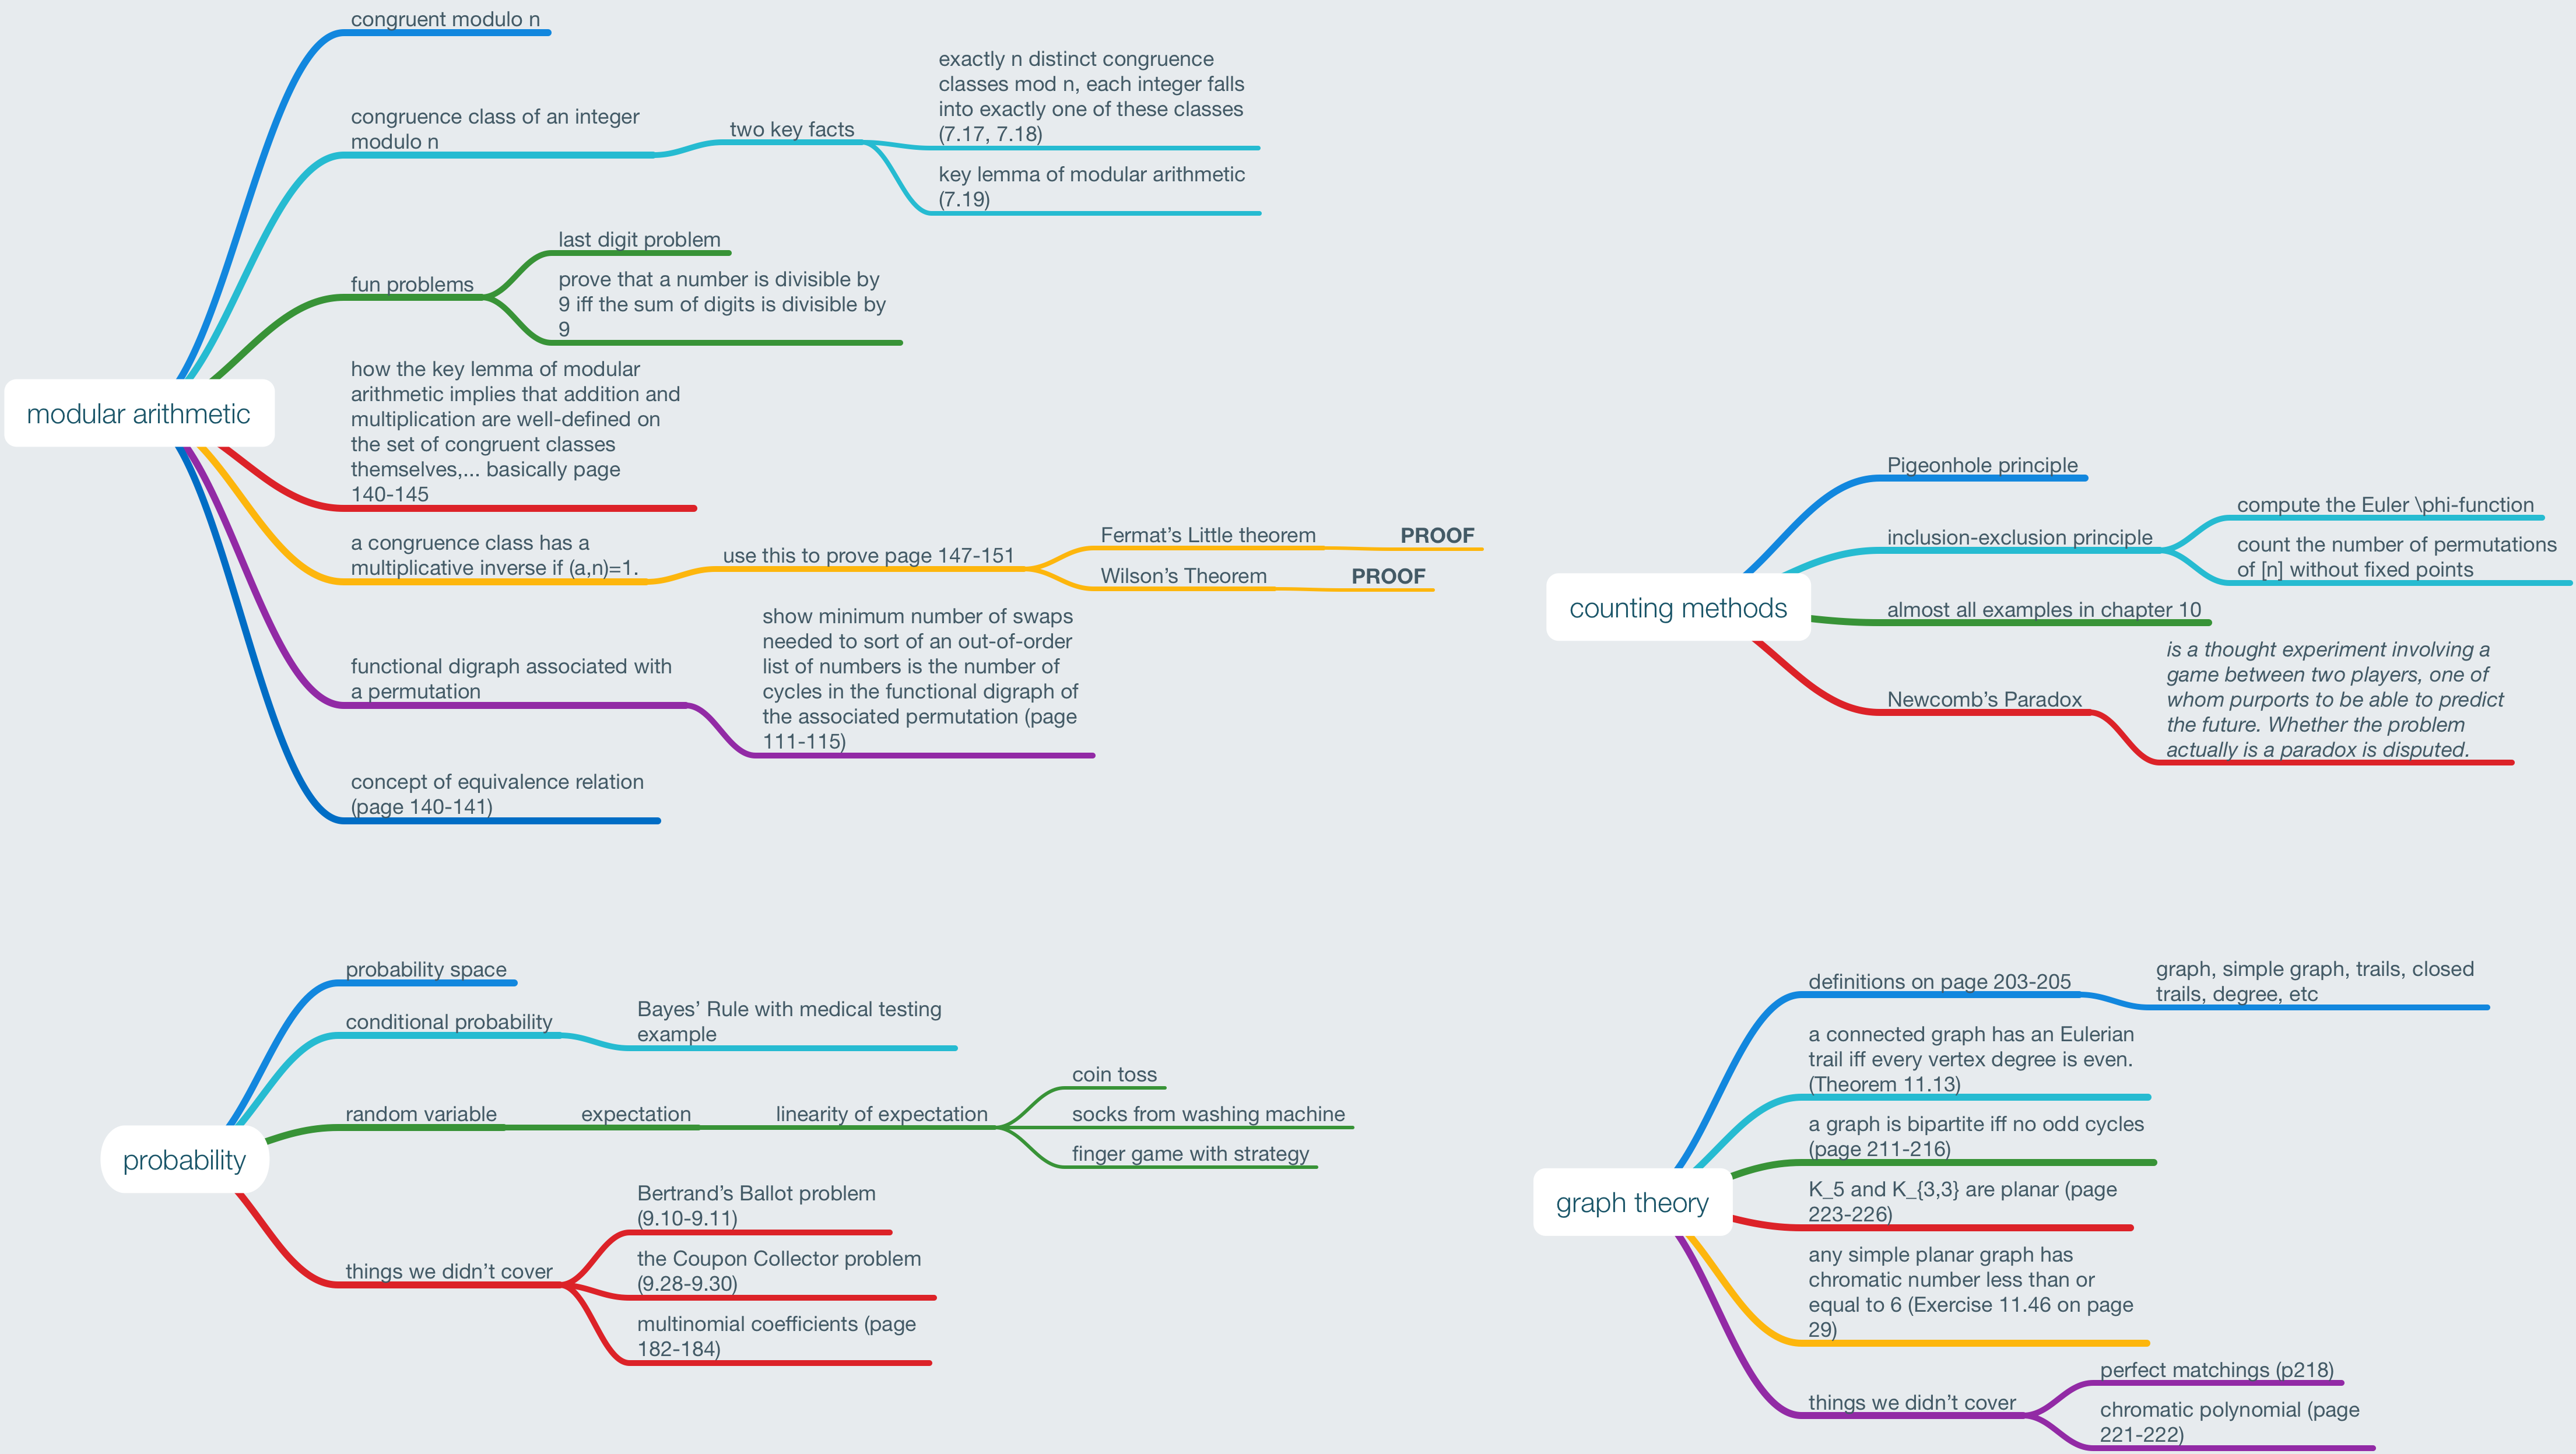
\includegraphics[width=\textwidth]{6222-mindmap}

\section{Modular Arithmetic}

\paragraph{Def:} An \textbf{equivalence relation} on a set $S$ is a relation $R$ on $S$ such that for all choices of distinct $x,y,z\in S$,
\begin{enumerate}
	\item $(x,x)\in R$ (\textbf{reflexive property})
	\item $(x,y)\in R \implies (y,x)\in R$ (\textbf{symmetric property})
	\item $(x,y)\in R, (y,z)\in R \implies (x,z)\in R$ (\textbf{transitive property})
\end{enumerate}

\paragraph{Def:} Given an equivalence relation on $S$, the set of elements equivalent to $x\in S$ is the \textbf{equivalent class} containing $x$.

\paragraph{Def:} The \textbf{functional digraph} of a function $f: A\rightarrow A$ consists of a point for each element of $A$ and, for each $x\in A$, an arrow from $x$ to $f(x).$ These points are vertices. \textbf{cycle...}

\paragraph{The number of transposition needed to sort the word form of a permutation of $[n]$ is $n-k$, where $k$ is the number of cycles in its cycle description.}

\paragraph{Proof:} Transposing two elements lying on distinct cycles combines their elements into a single cycle, while transposing two elements in the same cycle splits it into two cycles. When $f(i)=x$ and $f(j)=y$, transposing $x$ and $y$ yields $f'$ with $f'(i)=y$ and $f'(j)=x$; elsewhere $f$ and $f'$ agree. If $x$ and $y$ are in distinct cycles $x\cdots i$ and $y\cdots j$ of $f$, then the transposition yields the cycles $x\cdots y\cdots$ of $f$, then $f'$ has distinct cycles $x\cdots j$ and $y\cdots i$ on these elements.

By this claim, each transposition changes the number of cycles by one--up or down. The identity permutation consists of $n$ cycles of length $1$. Thus a permutation with $k$ cycles needs at least $n-k$ transpositions to reach the identity.

\paragraph{Def:} Given $n\in\mathbb{N^+}$, the integers $x$ and $y$ are \textbf{congruent modulo} $n$ if $x-y$ is divisible by $n$ as $x\equiv y\mod n$. $n$ is the \textbf{modulus.}

\paragraph{7.16. Theorem:} For every $n\in\mathbb{N}$, congruence modulo $n$ is an equivalence relation on $\mathbb{Z}$.

\paragraph{Def:} The equivalence classes of the relation ``congruence modulo $n$'' on $\mathbb{Z}$ are the \textbf{remainder classes} or \textbf{congruence classes} modulo $n$. The set of congruence classes is written as $\mathbb{Z}_n$ or $\mathbb{Z}/n\mathbb{Z}$.

\paragraph{7.18. Key fact:} There are $n$ remainder classes modulo $n$; for $0 \leq r < n$, the $r$th class in $\mathbb{Z}_n$ is $\{kn+r: k\in\mathbb{Z}\}$.

Observe that $\overline{0}, \overline{1},\dots, \overline{n-1}$ are clearly distinct congruence classes. If $0\leq i<j\leq n-1$, then $i-j$ can't be divisible by $n$ (too close!).

By definition $a\equiv b\mod n$ iff $a-b$ is divisible by $n$. The Division Algorithm yields unique integers $k,r$ such that $a=kn+r$ and $0\leq r<n$; here $r$ is the remainder upon division by $n$. If $a=kn+r$ and $b=ln+s$ with remainder $r, s\in\{0,\dots, n-1\}$, then $n|(a-b)$ iff $r-s=0$. Hence $a\equiv b\mod n$ iff $a$ and $b$ have the same remainder ``modulo $n$''. This justifies our description of the classes.

\paragraph{7.19. Lemma:} If $a\equiv r\mod n$ and $b\equiv s\mod n$, then $a+b\equiv r+s \mod n$ and $a\cdot b\equiv r\cdot s \mod n$.

\paragraph{Proof:} Let $a=kn+r$ and $b=ln+s$ where $k,l\in\mathbb{Z}\dots$

\paragraph{7.27. (an IMPORTANT) Lemma:} If $a$ and $n$ are relatively prime integers, then multiplication by $a$ defines a bijection from $\mathbb{Z}_n-\{0\}$ to itself; equivalently, multiplication by $a$ permutes the nonzero congruence classes.

\paragraph{Proof:} Since $a$ and $n$ are relatively prime, $0,a,2a,\dots, (n-1)a$ all have different remainders modulo $n$. Since $0$ has remainder $0$, the others are nonzero. Since they are distinct, the list defines an injection from $\mathbb{Z}_n -\{0\}$ to itself. Since the set is finite, this injection is a bijection.

\paragraph{7.28. Corollary:} If $a$ and $n$ are relatively prime integers, then solutions to $ax\equiv 1\mod n$ exists and lie in a single congruence class. In the language of $\mathbb{Z}_n$, the class $\overline{x}$ is the \textbf{multiplicative inverse} of $\overline{a}$.

\paragraph{Quick Proof:} By Euclidean algorithm: $\exists\ k, l\in \mathbb{Z}$ s.t. $ka+ln=1\iff ka\equiv 1\mod n$.

\paragraph{Def:} When some power of $a$ is congruent to $1$ modulo $p$, the \textbf{order} of $a$ (in $\mathbb{Z}_p$) is the least $k$ such that $a^k\equiv 1\mod p$.

\paragraph{7.34. Lemma:} Let $p$ be prime, and suppose that $a\not\equiv 0\mod p$. For $x\in\mathbb{Z}_p$, let $S_x=\{x,xa,xa^2,\dots\}$. There is a positive integer $k$ such that, for all $x\not=0$, the set $S_x$ consists of exactly $k$ elements.

\paragraph{7.35. Lemma:} If $R$ is the relation on $\mathbb{Z}_p$, defined by $(x,y)\in R$ iff $y\equiv xa^j\mod p$ for some nonnegative integer $j$, then $R$ is an equivalence relation.

\paragraph{$\spadesuit$ 7.36. Theorem (Fermat's Little Theorem):} If $p$ is prime and $a$ is not a multiple of $p$, then $a^{p-1}\equiv 1\mod p$.

\paragraph{Proof:} Let $k$ be the order of $a$ in $\mathbb{Z}_p$.

In the equivalence relation $R$ defined in Lemma 7.35, the equivalence class containing $0$ is $\{0\}$. The remaining classes partition $\mathbb{Z}_p-\{0\}$. The equivalence class $S_x$ containing $x$ consists of all classes obtainable from $x$ by multiplying a power of $a$. By Lemma 7.34, $S_x$ has size $k$. Thus $R$ partitions $\mathbb{Z}_p-\{0\}$ into sets of size $k$, and $p-1$ is a multiple of $k$. Thus

\[a^{p-1}=a^{mk}=(a^k)^m\equiv 1^m\equiv 1\mod p\]

\paragraph{7.39. Corollary:} If $p$ is prime and $a\in\mathbb{Z}$, then $a^p\equiv a\mod p$.

\paragraph{$\spadesuit$ 7.43. Lemma:} If $p$ is prime and $a\in\mathbb{N}$, then $a^2\equiv 1\mod p$ iff $a\equiv 1\mod p$ or $a\equiv -1\mod p$.

\paragraph{Proof:} If $a^2\equiv 1$, then $p$ divides $a^2-1$, which equals $(a+1)(a-1)$. When a prime divides a product, it must divide one of the factors. Hence $p$ divides $a+1$ or $a-1$, yielding $a\equiv -1\mod p$ or $a\equiv 1\mod p$. Conversely, if $a$ is one of these classes, then $p$ divides $(a+1)(a-1)$, and $a^2$ is in the same congruence class as $1$.

\paragraph{$\spadesuit$ 7.44. Theorem (Wilson's Theorem):} $(p-1)!\equiv -1\mod p$ for $p$ prime.

\paragraph{Proof:} This holds for $p=2$ because $1\equiv -1\mod 2$. Consider $p>2$. For each $1\leq i\leq p-1$, there is exactly one $i'$ in $[p-1]$ such that $ii'=1$ by Lemma 7.27. By Lemma 7.43, the numbers from $2$ through $p-2$ form disjoint pairs of inverses. Hence $\prod^{p-2}_{i=2}i\equiv 1\mod p$, and $\prod^{p-1}_{i=1}i\equiv p-1\equiv -1\mod p$.

\paragraph{Ex (``casting out nines''):} An integer is divisible by $9$ iff the sum of its decimal digits is divisible by $9$. Since $10$ is congruent to $1\mod 9$, every nonnegative power of $10$ is also congruent to $1 \mod 9$. Therefore,

\[\sum_{n\geq 0}a_n10^n\equiv \sum_{n\geq 0}1^n\equiv \sum_{n\geq 0}a_n\mod 9\]

\section{Probability}

\paragraph{Def:} A finite \textbf{probability space} is a finite set $S$ together with a function $P$ defined on the subsets of $S$ (called \textbf{events}) such that
\begin{enumerate}
	\item For $A\subseteq S, 0\leq P(A)\leq 1$,
	\item $P(S)=1$, and
	\item If $A,B$ are disjoint subsets of $S$, then $P(A\cup B)=P(A)+P(B)$.
\end{enumerate}

\paragraph{Def:} Conditional probability with $P(B)\not=0$:

\[P(A|B)=\frac{P(A\cap B)}{P(B)}\]

\paragraph{Def:} Events $A, B$ are \textbf{mutually exclusive} if $A\cap B=\varnothing$. They are \textbf{independent} if $P(A\cap B)=P(A)\cdot P(B)$.

\paragraph{Example of tossing coins:} ... since there are ${n\choose k}$ lists having $k$ heads, the probability of the event ``obtaining $k$ heads'' is ${n\choose k}p^k(1-p)^{n-k}$.

\paragraph{9.18. Proposition (Bayes' Formula):} Let $B_1,\dots ,B_k$ be mutually exclusive events whose probabilities $b_i=P(B_i)$ are known and sum to $1$. If $A$ is an event such that the conditional probabilities $a_i=P(A|B_i)$ are known, then

\[P(B_i|A)=\frac{P(B_i\cap A)}{P(A)}=\frac{P(A\cap B_i)}{\sum_jP(A\cap B_j)}=\frac{a_ib_i}{\sum_ja_jb_j}\]

\paragraph{Def:} Let $S$ be a finite probability space. A \textbf{random variable} is a function $X:S\rightarrow \mathbb{R}$. Each level set $I_X(k)$, the subset of $S$ on which $X$ takes the value $k$, is an event. We write $P(X=k)$ for the probability of this event. The \textbf{expectation} or \textbf{expected value} of $X$, written $E(X)$ is $\sum_kk\cdot P(X=k)$. In terms of individual points in the space, we also write

\[E(X)=\sum_{a\in S}X(a)P(a)\]

\paragraph{9.25. Proposition (Linearity of Expectation):} Let $X$ and $X_1,\dots, X_n$ be random variables on a finite probability space.
\begin{enumerate}
	\item For $c\in\mathbb{R}, E(cX)=cE(X)$.
	\item $E(X_1+\cdots +X_n)=E(X_1)+\cdots +E(X_n)$.
\end{enumerate} 

\paragraph{Proof:}

\[E(cX)=\sum_{a\in S}cX(a)=c\sum_{a\in S}X(a)=cE(X)\]

\[E(X)=\sum_{a\in S}X(a)P(a)=\sum_{a\in S}\left[\sum^n_{i=1}X_i(a)\right]P(a)=\sum^n_{i=1}\left[\sum_{a\in S}X_i(a)P(a)\right]=\sum^n_{i=1}E(X_i)\]

\paragraph{Application (Evil Laundry Machine):} $n$ pairs of socks in machine, spits out a random subset of $k$ socks. How many pairs of socks do we expect to see?

total outcomes = ${2n \choose k}$, $X$ is defined as the number of complete pairs in a particular subset, $X_i$ be the result that $i$th pair comes out. The subsets of size $k$ is ${2n-2 \choose k-2}$

\[E(X_1)=1\cdot P(X_1=1)+0\cdot P(X_1=0) = \frac{{2n-2\choose k-2}}{{2n\choose k}}\]

Then we sum them up by multiplying it by $n$.

\paragraph{Application (Finger Game):} ...

\section{Two Counting Methods}

\paragraph{10.1. Theorem (Pigeonhole Principle)}: Placing more than $kn$ objects into $n$ classes puts more than $k$ objects into some class.

\paragraph{10.12 Theorem (Inclusion-Exclusion Principle):} Given a universe $U$ of items and subsets $A_1, \dots, A_n$ of the items, the number of $N_{\varnothing}$ of items belonging to none of the subsets is given by

\[N_{\varnothing}=\sum_{S\subseteq [n]}(-1)^{|S|}\bigg|\bigcap_{i\in S}A_i\bigg|.\]

\paragraph{Ex: Euler totient.} Suppose that $m$ has $n$ distinct prime factors $p_1,\dots, p_n$. $U=[m]$, define $A_i$ to be the multiples of $p_i$. For the intersection of the sets indexed by the elements of $S\subseteq [n]$, we have $\big|\cap_{i\in S}A_i\big|=m/\prod_{i\in S}p_i$. Apply principle,

\[\phi(m)=N_{\varnothing}=\sum_{S\subseteq [n]}(-1)^{|S|}\bigg|\cap_{i\in S}A_i\bigg|=\sum_{S\subseteq [n]}(-1)^{|S|}\frac{m}{\prod_{i\in S}p_i}.\]

\paragraph{Ex: Derangements.} Count the permutations of $[n]$ s.t. no $i$ is in position $i$. An instance of $i$ in position $i$ is a fixed point; the derangements are the permutations with no fixed points. $A_i$ is defined to be a permutation of $i$th point fixed. Let $|S|=k, S\subseteq [n]$, so $\big|\cap_{i\in S}A_i\big|=(n-k)!$. Also there are ${n\choose k}$ choices of $S$ with size $k$, so

\[D_n=N_{\varnothing} = \sum^n_{k=0}(-1)^k{n\choose k}(n-k)!\]

\paragraph{Ex: Rolling dice.} Roll a die $n$ times, what's the prob that every $1$ to $6$ appears at least one?

\[{6\choose 0}\cdot \frac66^n-{6\choose 1}\left(\frac{5}{6}\right)^n+{6\choose 2}\left(\frac{4}{6}\right)^n-{6\choose 3}\left(\frac{3}{6}\right)^n+{6\choose 4}\left(\frac{2}{6}\right)^n-{6\choose 5}\left(\frac{1}{6}\right)^n\]

And this number needs to be divided by $6^n$.

\section{Graph Theory}

\sout{Hello World}

\paragraph{Def:} A \textbf{graph} $G$ is a triple consisting of a finite \textbf{vertex set} $V(G)$, a finite \textbf{edge set} $E(G)$, and a function $h_G$ that assigns to each edge $e\in E(G)$ an unordered pair of vertices. When $h_G(e)=\{u, v\}$ , we say that $u,v$ are endpoints of $e$ and that $e$ is incident to $u,v$. A graph $G$ is \textbf{simple} if the function $h_G(e)$ is injective. In this case, we write $e=uv$ instead of $h_G(e)=\{u, v\}$. (i.e. there is at most one edge between $u,v$.)

\paragraph{Def:} The \textbf{degree} of a vertex $x\in V(G)$, written $d(x)$, is the number of edges in $G$ incident to $x$. A \textbf{subgraph} of a graph $G$ is a graph $H$ such that $V(H)\subseteq V(G)$ and $E(H)\subseteq E(G)$; we also require $h_H(e)=h_G(e)$ for $e\in E(H)$. When $H$ is a subgraph of $G$, we write $H\subseteq G$ and say `` $G$ contains $H$''.

\paragraph{Def:} A \textbf{trail} in a graph $G$ is a list $v_0, e_1,v_1,e_2, \dots, e_k, v_k$ that alternates between vertices and edges, s.t. $h_G(e_i)=v_{i-1}v_i$ for all $i$, and $e_1,\dots, e_k$ are distinct. The \textbf{length} of a trail is the number of edges. A $u,v$-\textbf{trail} is a trail with first vertex $u$ and last vertex $v$; these are its \textbf{endpoints}.

A trail is \textbf{closed} if its endpoints are equal or if it has length 0. A trail in a graph is \textbf{maximal} if it is not a sublist of a longer trail. A graph is \textbf{Eulerian} if it has closed trail containing all its edges.

\paragraph{11.12. Lemma:} If every vertex of a graph $G$ has even degree, then every maximal trail in $G$ is closed.

\paragraph{Proof:} Since a trail  contributes degree two when it passes through a vertex, a non-closed trail uses an odd number of edges at the endpoints. If the endpoint has even degree, then a non-closed trail can be extended. We have proved the contrapositive of the claim.

\paragraph{$\spadesuit$ 11.13. Theorem:} A graph $G$ is Eulerian iff each vertex has even degree and each edge is reachable from every other.

\paragraph{Proof:} One way proved in Lemma 11.12.

Suppose that $G$ satisfies the conditions. Let $T$ be a maximal trail in $G$; by Lemma 11.12, $T$ is closed. If $T$ does not include all of $E(G)$, let $G'$ be the subgraph obtained from $G$ by deleting $E(T)$. Since every edge of $G$ is reachable from every other, there is a trail in $G$ that starts with an edge of $T$ and contains an edge of $G'$; let $e$ be the first edge of $G'$ on this trail, and let $v$ be the vertex it follows.

Since $T$ has even degree at every vertex, every vertex also has even degree in $G'$. Let $T'$ be a maximal trail in $G'$ beginning from $v$ along $e$. By Lemma 11.12, $T'$ is closed and ends at $v$. Hence we may incorporate $T'$ to obtain a trail properly containing $T$. This contradicts the maximality of $T$, so we conclude that $T$ already contains all edges of $G$.

\paragraph{11.14. Theorem (Degree-sum Formula):} If $G$ is a graph with $m$ edges, then $m=\frac{1}{2}\sum_{v\in V(G)}d(v)$.

\paragraph{Proof:} Summing the degrees counts each edge twice, since each edge has two endpoints and contributes to the degree of each endpoint.

\paragraph{11.16. Corollary:} Every graph has an even number of vertices of odd degree.

\paragraph{Proof:} By the Degree-sum Formula, the sum of the degrees is even. Hence the sum must have an even number of odd contributions.

\paragraph{Def:} An \textbf{isomorphism} from a simple graph $G$ to a simple graph $H$ is a bijection $f:V(G)\rightarrow V(H)$ such that $uv\in E(G)$ iff $f(u)f(v)\in E(H)$. We say ``$G$ is isomorphic to $H$'' written $G\cong H$, if there is an isomorphism from $G$ to $H$. The set of pairs $(G, H)$ such that $G$ is isomorphic to $H$ is the \textbf{isomorphism relation}.

\paragraph{Def:} Vertices $u$ and $v$ in a graph $G$ are adjacent and are \textbf{neighbours} if they are the endpoints of an edge. The \textbf{adjacency relation} of $G$ (defined on $V(G)$) is the set of ordered pairs $(u, v)$ s.t. $u$ and $v$ are adjacent.

\paragraph{11.20. Proposition:} The isomorphism relation is an equivalence relation on the set of simple graphs.

\paragraph{Proof:} The identity map on $V(G)$ is an isomorphism from $G$ to itself. If $f: V(G)\rightarrow V(H)$ is an isomorphism from $G$ to $H$, then $f^{-1}$ is an isomorphism from $H$ to $G$. If $f: V(F)\rightarrow V(G)$ and $g:V(G)\rightarrow V(H)$ are isomorphisms, then $g\circ f$ is a bijection from $V(F)$ to $V(H)$ that preserves the adjacency relation and hence is an isomorphism from $F$ to $H$. Thus the isomorphism relation is reflexive, symmetric, and transitive.

\paragraph{Def:} The \textbf{complement} $\overline{G}$ of a simple graph $G$ is the graph with vertex set $V(G)$ and edge set $\{\{u,v\}: uv\not\in E(G)\}$.

\paragraph{Def:} A \textbf{path} is a simple graph whose vertices can be listed in an order so that two vertices are adjacent iff they are consecutive in the list. The \textbf{endpoint}s of a path are the first and last vertices in such a list. A $u,v$-\textbf{path} is a path with endpoints $u$ and $v$.

A \textbf{cycle} is a simple graph whose vertices can be place at distinct points of a circle s.t. two vertices are adjacent iff they appear consecutively on the circle.

The \textbf{length} of a path or cycle is its number of edges. We use $P_n$ and $C_n$, respectively, to denote any representative of the isomorphism class that is a path or cycle with $n$ vertices.

\paragraph{Def:} A graph $G$ is \textbf{connected} if for all $u, v\in V(G)$, there is a $u,v$-path in $G$ (otherwise, $G$ is disconnected). A \textbf{component} of $G$ is a connected subgraph of $G$ that is not contained in any other connected subgraph. An \textbf{isolated vertex} is a vertex with degree $0$.

\paragraph{11.33. Proposition:} If $P$ is a $u,v$-path and $P'$ is a $v,w$-path, then $P$ and $P'$ together contain a $u,w$-path.

\paragraph{11.36. Lemma:} If $e$ is an edge of a connected graph $G$, then $G-e$ is connected iff $e$ belongs to a cycle of $G$.

\paragraph{$\spadesuit$ 11.37. Lemma:} If every vertex of $G$ has degree at least two, then $G$ contains a cycle.

\paragraph{Proof:} Since $V(G)$ is finite, we can choose a maximal path $P$. Let $v$ be an endpoint of $P$. Since $d(v)\geq 2, v$ has a neighbour $u$ that is not a neighbor of $v$ on $P$. Since we cannot extend $P$ to reach a new vertex from $v$, the vertex $u$ already belongs to $P$, and the edge $vu$ completes a cycle with the $u,v$-portion of $P$.

\paragraph{Def:} A \textbf{tree} is a connected graph with no cycles. A \textbf{leaf} is a vertex of degree $1$. A \textbf{spanning tree} of a graph $G$ is a subgraph of $G$ that is a tree containing all vertices of $G$.

\paragraph{$\spadesuit$ 11.39. Lemma:} Every tree with at least two vertices has a leaf, and deleting a leaf from a tree yields a tree with one less vertex.

\paragraph{Proof:} Let $G$ be a tree with $n$ vertices, where $n\geq  2$. By the contrapositive of Lemma 11.37, a graph with no cycles has a vertex of degree less than two. Since $G$ is connected and has more than one vertex, it has no vertex of degree $0$, so it has a leaf $x$. Let $G'=G-x$.

We claim that $G'$ is a tree with $n-1$ vertices. We cannot create a cycle by deleting a vertex, so we need only show that $G'$ is connected. Consider distinct vertices $u,v\in V(G')$. Because $G$ is connected, there is a $uv$-path $P$ in $G$. Since internal vertices along a path have degree at least $2$, $P$ cannot contain $x$. Hence $P$ is contained in $G'$.

\paragraph{$\spadesuit$ 11.40. Theorem:} Every tree with $n$ vertices has $n-1$ edges.

\paragraph{Proof:} We use induction on $n$. A tree with $1$ vertex has no edges. For the induction step, we consider $n>1$ assume that trees with $n-1$ edges have $n-2$ vertices. If $G$ is a tree with $n$ vertices, then Lemma 11.39 yields a leaf $x$ and a tree $G'=G-x$ with $n-1$ vertices. By the induction hypothesis, $G'$ has $n-2$ edges. Since $x$ appears in only one edge, we conclude that $G$ has $n-1$ edges.

\paragraph{Def:} A set $S\subseteq V(G)$ is an \textbf{independent set} in a graph $G$ if $uv\not\in E(G)$ for all $u,v\in S$ ($S$ may be empty). A \textbf{bipartite graph} with \textbf{bipartition} $X, Y$ is a graph $G$ s.t. $V(G)=X\cup Y$ and $X,Y$ are disjoint (possibly empty) independent sets. We call $X$ and $Y$ the \textbf{bipartite set} or \textbf{parts} of the bipartition.

\paragraph{11.43. Proposition:} Every tree is bipartite.

\paragraph{Proof:} We use induction on the number of vertices. Lemma 11.39...

\paragraph{$\spadesuit$ 11.44. Theorem:} A graph is bipartite iff it contains no cycle of odd length.

\paragraph{Proof:} Use ``odd cycle'' of ``cycle of odd length'' to prove the condition is necessary.

Use proposition 11.43 to prove the sufficiency.

\paragraph{Def:} A \textbf{complete graph} is a simple graph in which every pair of vertices forms an edge. We use $K_n$ to denote the isomorphism class of complete graphs with $n$ vertices (or its representatives).

\paragraph{Def:} A $k$-\textbf{coloring} of a graph $G$ is a function $f:V(G)\rightarrow S$, where $S$ is a set of $k$ elements called \textbf{colors} (the colors need not all be used). A $k$-coloring is \textbf{proper} if no pair of adjacent vertices receive the same color. The \textbf{chromatic number} of $G$, written $\chi(G)$, is the minimum $k$ s.t. $G$ has a proper $k$-coloring.

\paragraph{Ex Coloring of generalized cycles}: $G_{n,k}$ is the graph obtained by making each point adjacent to the $k-1$ nearest points in each direction. The graph $G_{n,1}$ is an independent set, which is $1$-colorable. The graph $G_{n,2}$ is the ordinary cycle $C_n$, which has chromatic number $2$ when $n$ is even and $3$ when $n$ is odd.

\paragraph{11.53. Theorem:} If $n\geq k(k-1)$, then the chromatic number of the generalized cycle $G_{n,k}$ is given by

\[\chi(G_{n,k})=\begin{cases}
	k\ & \text{if $k$ divides $n$}\\
	k+1\ &\text{if $k$ does not divide $n$.}
\end{cases}\]

\paragraph{Def:} A \textbf{drawing} of a graph $G$ is a graph $H$ isomorphic to $G$ s.t. each vertex of $H$ is a point in $\mathbb{R}^2$ and each edge $e$ of $H$ with endpoints $u,v$ is a simple curve from $u$ to $v$. In a drawing of a graph, distinct edges $e_1$ and $e_2$ \textbf{cross} if they intersect other than at a common endpoint. A \textbf{planar graph} is a graph that has a drawing without crossings. Such a drawing is called a \textbf{plane graph}.

\paragraph{Def:} A \textbf{face} $F$ of a plane graph $G$ is a maximal path-connected subset of $\mathbb{R}^2$ that intersects no edge or vertex of $G$. An edge $e$ is in the \textbf{boundary} of $F$ if some segment with an endpoint in $F$ crosses $e$ and no other edge of $G$.

\paragraph{$\spadesuit$ 11.64. Theorem (Euler's Theorem):} If $G$ is a connected plane graph with $\textbf{v}$ vertices, $\textbf{e}$ edges, and $\textbf{f}$ faces, then $\textbf{v}-\textbf{e}+\textbf{f}=2$.

\paragraph{Proof:} We use (strong) induction on the number of cycles in $G$. If $G$ is connected and has no cycles, then $G$ is a tree and $\textbf{f}=1$. Since $\textbf{e}=\textbf{v}-1$ for a tree, we are done.

Otherwise, $G$ has a cycle $C$ containing an edge $e$. Because $C$ is a cycle, the Jordan Curve Thm implies that $e$ is on the boundary of two faces in $G$; one inside $C$ and one outside $C$. In the plane graph $G'=G-e$, these faces merge (including the points vacated by $e$) to form a single face.

Since $e$ belongs to a cycle, Lemma 11.36 implies that $G'$ is connected. Furthermore, $G'$ has fewer cycles than $G$, since every cycle in $G'$ appears in $G$, but $C$ appears in $G$ and not $G'$. Hence we can apply the induction hypothesis to $G'$; if its number of vertices, edges, and faces are $\textbf{v'}, \textbf{e'}, \textbf{f'}$, this yields $\textbf{v'}-\textbf{e'}+\textbf{f'}=2$. Since $\textbf{v}=\textbf{v'}, \textbf{e}=\textbf{e'}+1,\textbf{f}=\textbf{f'}+1$, then...

\paragraph{$\spadesuit$ 11.65 Theorem:} Every simple planar graph with $n\geq 3$ vertices has at most $3n-6$ edges. Every simple planar graph with $n\geq 3$ vertices has no $3$-vertex cycle has at most $2n-4$ edges.

\paragraph{Proof:} For $n=3$, both statements are true by inspection. Consider a maximal simple plane graph $G$ with $n\geq 4$. We may assume $G$ is connected, since otherwise we can add at least one edge. We can now use Euler's Formula to relate $\textbf{v}$ and $\textbf{e}$ if we can dispose of $\textbf{f}$. Since $G$ is simple, every face has at least three edges in its boundary. Every edge lies in the boundary of at most two faces. Summing the numbers of edges in the boundaries of the faces thus yields the inequality $2\textbf{e}\geq 3\textbf{f}$. Substituting this into $n-\textbf{e}+\textbf{f}=2$ yields $\textbf{e}\leq 3n-6$.

For the second statement, we check the graphs with $n=4$ individually. If also $G$ has no $C_3$ and $n\geq 5$, then each face of $G$ has at least 4 edges in its boundary. In this case the inequality becomes $2\textbf{e}\geq 4\textbf{f}$, and we obtain $\textbf{e}\leq 2n- 4$.

\paragraph{Ex $K_5$ and $K_{3,3}$:} Theorem 11.65 implies that $K_5$ has $\textbf{e}=10>9=3n-6$. Also for $K_{3,3}$ we have $\textbf{e}=9>8=2n-4$. Each graph can be drawn using only one crossing.

\paragraph{Kuratowski's Theorem:} A simple, connected graph $G$ is planar iff does not contain an expansion of $K_{3,3}$ or $K_5$ as a subgraph.

\paragraph{$\spadesuit$ Prove that every simple planar graph has a vertex of degree at most $5$, and use this to prove that every planar graph has chromatic number at most $6$.} Theorem 11.65 states that every simple planar graph $G$ with $n$ vertices has at most $3n-6$ edges. By the degree-sum formula, the degrees of our $G$ thus sum to at most $6n-12$. By the pigeonhole principle, some vertex has degree at most the average, which equals $6-12/n$. Thus some vertex has degree at most $5$.

Since multiple edges do not affect chromatic number, we only need consider simple planar graphs. We use induction on the number of vertices; every graph with at most $6$ vertices has chromatic number at most $6$. When $n>6$, we know that a simple planar graph $G$ with $n$ vertices has a vertex $x$ of degree at most $5$. Let $G'=G-x$. Since $G'$ is planar, the induction hypothesis implies that $G'$ has chromatic number at most $6$. Since at most five of the colors are used on the neighbors of $x$, there is some color available to use on $x$ to extend this to a proper $6$-coloring of $G$.

\end{document}